\scanpage{14}
\figure{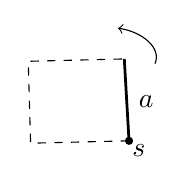
\begin{tikzpicture}[x=1cm,y=1cm]
\draw[dashed](1.25,.03)--(0,0)--(-.03,1.04)--(1.19,1.07);
\draw[line width=1pt](1.19,1.07)--(1.25,.03);
\fill(1.25,.03) circle (.052);
\node[right] at (1.25,.53){$a$}; \node[below right,inner sep=1pt] at (1.25,.03){$s$};
\draw[->](1.58,1.01)..controls (1.67,1.22) and (1.40,1.42)..(1.11,1.46);
\end{tikzpicture}}
je lui associe la rotation du carré qui transforme $s$ en le deuxième sommet de $a$. On vérifie que avec ces conventions, la formule $\varpi c d=1$ est bien la formule qui exprime que $\mathcal{R}_{\varpi}\subset \mathcal{R}$ contient l'image inverse par $\mathcal{R}\unsure{\longrightarrow|\text{---}}\mathcal{R}/\underline a$ de l'élément $(c,d)$ de $\mathcal{R}/\underline a$. Le fait que si on exprime la $=$ relation pour le carré dual, on semble obtenir le résultat opposé, provient du fait que si on identifie le $=$ ensemble $\mathcal{R}$ à l'ens. des repères de $Q$ \uline{et} de $Q^{\unsure{o|0|\circ}}$, \deleted{les} \deleted{deux} \inserted{et} le $=$ groupe $\unsure{\mathfrak{D}|\mathscr{D}}$ à $\mathrm{Aut}\,Q$ \uline{et} à $\mathrm{Aut}(Q^o)$ (ce qui n'est possible canoniquement que d'une seule façon \inserted{\unsure{raisonnable|vraisemblable}}, i.e. ce n'est pas une question de choix de conventions \ldots) alors une $=$ \deleted{partie} \inserted{classe} $\mathcal{R}'$ dans $\mathcal{R}$ \deleted{\unsure{comme|commune}} (pour la relation d'équivalence \unsure{de|del} l'orientation), considérée comme définissant une orientation de $Q$ \uline{et} une orientation de $Q^o$, définit deux orientations \uline{opposées}, en ce sens que les autom. de rotations qu'il définit via un repère $(s,a)$, suivant qu'il est regardé comme rep. de $Q$ ou rep. de $Q^o$, \unsure{sont|soit} \uline{opposés} l'un de l'autre : transformer $s$ en $s'$ ou $a$ en $a'$ se fait par deux rotations \uline{opposées}.
\figure{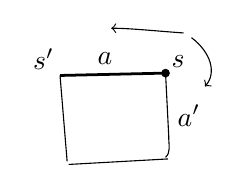
\begin{tikzpicture}[x=1cm,y=1cm]
\draw(0,.08)--(-.09,1.17) (1.25,1.20)--(1.29,.41)..controls (1.29,.27) and (1.32,.20)..(1.25,.13) (1.28,.11)--(.02,.04);
\draw[line width=1.0pt](-.09,1.17)--(1.25,1.20);
\fill(1.25,1.20) circle (.055);
\node[above left,inner sep=2pt] at (-.09,1.17){$s'$}; \node[above right,inner sep=2pt] at (1.25,1.20){$s$};
\node[above] at (.48,1.19){$a$}; \node[right] at (1.28,.66){$a'$};
\draw[->](1.48,1.71)..controls (1.18,1.73) and (.80,1.77)..(.56,1.77);
\draw[->](1.58,1.65)..controls (1.83,1.46) and (1.90,1.20)..(1.75,1.03);
\end{tikzpicture}}
% archive sheet number: 13
